\chapter{Relative Indexing Design}
While the Closest Finger Design does greatly simplify the task of handling up to ten simultaneous touches, it does so by avoidance. By restricting each sprite to only being able to listen to one touch at a time, the Closest Finger Design eludes having to handle ten touches within the same script. Even though this approach is reasonable, there are other potential strategies for simplification without such a restriction.

For example, one natural way to think about handling the up to ten simultaneous touches is to think of them as ten persistent touch-objects, among which all touch inputs are distributed. Since there can be at most ten simultaneous touch inputs, ten touch-objects are enough to handle all touch inputs made throughout the execution of any project. The big question with such a design becomes: What is the best way to distribute the touch inputs amongst the ten touch-objects?

In this second multi-touch interaction set design, which I have named the \emph{Relative Indexing Design}, the persistent touch-objects are indexed $1$ through $10$ and represent the status of the touch inputs with matching indices. The touch inputs are indexed relative to the other concurrent touches in order of initiation from $1$ to the number of current touches. Since touches are (as the design's name implies) indexed relatively, a touch's associated index (and, thus, associated persistent touch-object) can  be subject to change. For example, a touch that was the third-oldest current touch (meaning it has an associated index of 3) can become the oldest current touch (meaning an associated index of 1) if the two older current touches are lifted. While this manner of indexing is intuitive, it has a few quirks that can lead to many unforeseen bugs in the development of seemingly simple projects.

In this chapter, I will first specify the Relative Indexing Design and then follow up by evaluating the design on the three iterations of case projects that I described in Chapter 3.

\section{Interaction Set Specification}

The Relative Indexing Design consists of nine touch blocks, only one of which is wholly original to this thesis: the ``number of fingers" block (Figure \ref{Number_Of_Fingers}). As the name implies, the ``number of fingers" block produces a value ranging from \emph{0} to \emph{10}, representing the number of fingers on the tablet at the time of evaluation. Since most tablets can only recognize up to ten simultaneous touches, the ``number of fingers" block will return the value of \emph{10} whenever there are 10 or more touches.

\begin{figure}
\centering

\includegraphics{images/Number_Of_Fingers.PNG}
\caption[The ``number of fingers" Block]{The ``number of fingers" block.}
\label{Number_Of_Fingers}
\end{figure}

The remaining eight touch blocks in the Relative Indexing Design are the same in appearance as the unextended Closest Finger Design interaction set, with the exception that each of the Relative Indexing Design blocks has an added numerical parameter (see left side of Figure \ref{Relative_Indexing_Design_Block_Set}). This parameter is used to select the index (ranging from 1 to 10) of the desired touch of interest.\footnote{Note that in these blocks I again use the term ``finger" instead of touch. Although this terminology could lead some novices into thinking that the touch indices correspond to particular fingers (e.g., finger 5 always refers to the user's left thumb), I believe it is still beneficial to use the concrete term ``finger," rather than the abstract term ``touch."}
The parameter is a drop-down menu with values ranging from 1 to 10, but it is also a slot that can be filled with a function block (see right side of Figure \ref{Relative_Indexing_Design_Block_Set}). If the inserted function block returns a value other than an integer between 1 and 10, the value gets defaulted to 1, so as to avoid throwing errors.

\begin{figure}
\centering
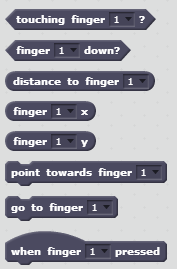
\includegraphics{images/Relative_Indexing_Design_Block_Set.PNG}
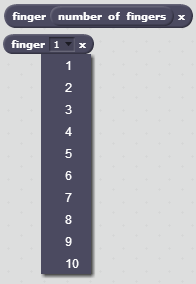
\includegraphics{images/Relative_Indexing_Design_Block_Dropdown_Show.PNG}
\caption[Remaining Eight Blocks In The Relative Indexing Design Interaction Set]{On the left are the remaining eight blocks in the Relative Indexing Design interaction set.  On the right there are two examples of the ``finger (\emph{index}) x" block: one with the drop-down menu opened and the other with an inserted function block.}
\label{Relative_Indexing_Design_Block_Set}
\end{figure}

Of these eight remaining touch blocks, only two, the ``finger (\emph{index}) down?" and ``when finger (\emph{index}) pressed" blocks, are not affected by the location of the touch inputs, so I will quickly explain them first. The ``finger (\emph{index}) down?" block is a simple Boolean function block that returns a value of \emph{true} if the touch with the index of (\emph{index}) is currently down and a value of \emph{false} otherwise. By the nature of relative indexing, this is the equivalent of determining whether
there are at least (\emph{index}) touches currently pressed on the tablet. As a result, the ``finger (\emph{index}) down?" block is redundant, since this value can be determined using the ``number of fingers" block along with some logic blocks. Even so, the ``finger (\emph{index}) down?" block is a worthwhile shortcut, because it can become tedious to determine the value repeatedly.

The ``when finger (\emph{index}) pressed" block is a simple trigger block that is closely related to the ``finger (\emph{index}) down?" function block. The ``when finger (\emph{index}) pressed" block is triggered at the moment the finger with the index of (\emph{index}) is pressed. In other words, the ``when finger (\emph{index}) pressed" block executes its connected stack at the moment the number of touches on the tablet increases from (\emph{index-1}) to (\emph{index}). Like its Closest Finger Design analogue, the ``when finger (\emph{index}) pressed" block restarts the execution of its connected stack when it is triggered for a second time before finishing the first execution.

The final six blocks, ``touching finger (\emph{index})?", ``distance to finger (\emph{index})," ``point towards finger (\emph{index})," ``go to finger (\emph{index})," ``finger (\emph{index}) x," and ``finger (\emph{index}) y," behave the same as their Closest Finger Design counterparts except that their location of interest is the current location of the touch with the index of (\emph{index}) instead of the sprite's closest touch. When (\emph{index}) is less than or equal to the current number of touches (i.e., the ``finger (\emph{index}) down?" block evaluates to \emph{true}), the location touch with the index of (\emph{index}) is simply the location of the (\emph{index})th-longest-lasting touch currently on the tablet. Otherwise, when (\emph{index}) is greater than the current number of touches (i.e., the ``finger (\emph{index}) down?" block evaluates to \emph{false}), the location of the touch with the index of (\emph{index}) remains at its last location. Again, prior to all touches, the fingers of all indices have the arbitrary, default  location of $\{0,0\}$.

\section{Evaluation}

Due to the functionality of the Relative Indexing Design being fairly straightforward, many of the simpler multi-touch interactions can be implemented intuitively. However, as projects get more complicated, the limitations of the Relative Indexing Design become evident.

\subsection{Low Floor}
For projects that assume a maximum of one touch on the screen at a time, the  Relative Indexing Design has the capability to behave identically to the Closest Finger Design. When there is only one touch on the screen, that touch is every sprite's closest touch. Similarly, the relative index of the single touch will, by definition, always be 1. Thus, both the basic one-player Pong game and the one-finger painting project can be implemented using the Relative Indexing Design in essentially the same way as they were implemented in the Closest Finger Design in the previous chapter (Figure \ref{LowFloorRID}).

\begin{figure}
\centering
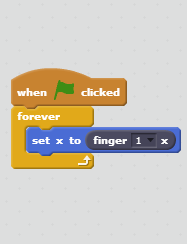
\includegraphics{images/OnePlayerPongRID.PNG}
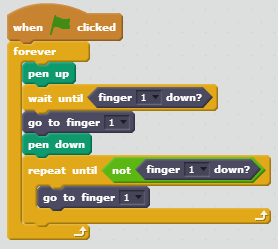
\includegraphics{images/OneFingerPaintingRID.PNG}
\caption[Sample Relative Indexing Design Scripts for Low Floor Case Projects]{On the left is the Relative Indexing Design script for the one-player Pong game paddle controls.  On the right is the script for one-finger painting.}
\label{LowFloorRID}
\end{figure}

Although  these low floor case projects can be implemented using the Relative Indexing Design as easily as with the Closest Finger Design, the latter does a slightly better job of lowering the floors. The parameter in the Relative Indexing Design blocks does not provide any added functionality for single-touch projects, so it can only contribute to potential confusion.

\subsection{Middle Height}

The middle height case projects are not particularly well suited for the Relative Indexing Design. To begin with, the Relative Indexing Design does not filter the touch inputs for the closest touch (unlike the Closest Finger Design). As a result, implementing the basic one-player Pong game is slightly more laborious, even though it is still a relatively straightforward process (Figure \ref{BasicTwoPlayerPongRID}). Since we have the assumption that there will be at most two simultaneous touches, both paddles only have to listen to the touches with indices 1 or 2. For each paddle, it does not matter whether a touch was the first or the second touch made. Thus, the paddle's script must forever repeat the process of checking both touches and follow the y-coordinate of the touch that is within the paddle's control range (if there is such a touch).

\begin{figure}
\centering
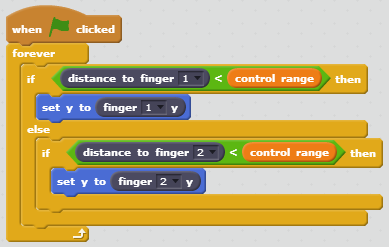
\includegraphics{images/BasicTwoPlayerPongRID.PNG}
\caption[Sample Relative Indexing Design Script For Basic Two-Player Pong]{Here is a sample script for controlling the paddle in a basic two-player Pong game using the Relative Indexing Design.}
\label{BasicTwoPlayerPongRID}
\end{figure}

This implementation is fairly easy to follow when presented, but has a few subtleties that can be tricky for Scratchers to figure out. For example, if a Scratcher is not careful, it is possible to fall victim to the bug of having the paddle stuck ``following" an already lifted touch. While these bugs can be tricky for beginners, they are relatively concrete as far as bugs go, so I am confident that Scratchers (especially with the help of the supportive Scratch community) will be able to overcome them and learn from them. 

Similarly, implementing the two-finger painting project using the Relative Indexing Design also has a few subtle pitfalls. However, unlike the case for the basic one-player Pong game, the bugs that arise when implementing the two-finger painting project are very difficult to overcome. Naive intuition would suggest that each paintbrush sprite wait for and subsequently follow a different indexed touch. In other words, one paint brush would follow the first touch when it occurs and the second paint brush would follow the second touch when it occurs (left side of Figure \ref{NaiveTwoFingerPaintingRID}).

\begin{figure}
\centering
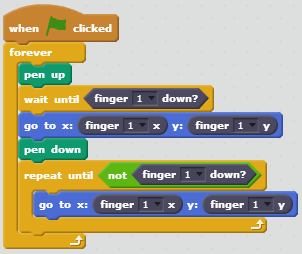
\includegraphics[width=0.415\textwidth]{images/NaiveTwoFingerPaintingRID.PNG}
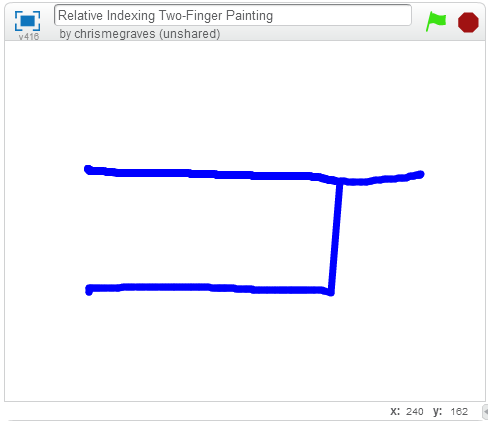
\includegraphics[width=0.4\textwidth]{images/IndexTransferLineBug.PNG}
\caption[Sample Naive Script For Two-Finger Painting Using the Relative Indexing Design ]{On the left is a sample naive paintbrush script using the Relative Indexing Design. On the right is the result of the bug caused by the touch index transferring.}
\label{NaiveTwoFingerPaintingRID}
\end{figure}

This control scheme works for the most part, but there is a pernicious bug for which there is no simple solution. The bug occurs when there are two touches simultaneously on the tablet, and the touch with index 1 (i.e., the first touch) is lifted before the touch with index 2 (i.e., the second touch). At this moment, the paintbrush following the second created touch stops following it, because ``finger (2) down?" would evaluate to \emph{false}. Also, the paintbrush following the first touch, would then start to follow the second touch, since its index changed from 2 to 1. This transfer is fine, but the problem is that the paintbrush following the first touch does not know to lift up its pen before starting to follow the second paintbrush, leading to an unintentional line in the user's painting (e.g., right side of Figure \ref{NaiveTwoFingerPaintingRID}). 

There are reasonable solutions (e.g., left side of Figure \ref{WaryTwoFingerPaintingRID}) to the bug that prevent the unintentional line from appearing, but they result in small gaps in the finger painting lines (e.g., right side of Figure \ref{WaryTwoFingerPaintingRID}). Furthermore, even these imperfect solutions pose a considerable challenge to experienced Scratchers. A ``perfect," practical implementation for multi-finger painting cannot be done using the Relative Indexing Design, because some data will be lost when the touch index transfers occur. This loss of data is due in part to the fact that there is no sure way to differentiate between two similar but importantly distinct events: the event in which the first touch is lifted before the second and the event in which the second touch is lifted before the first. That being said, reasonable assumptions can be made by comparing touch locations, as was the case for the Closest Finger Design. 

\begin{figure}
\centering
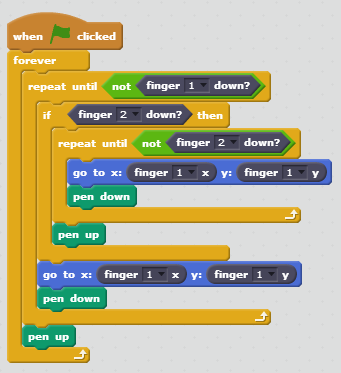
\includegraphics[width=0.4\textwidth]{images/WaryTwoFingerPaintingRID.PNG}
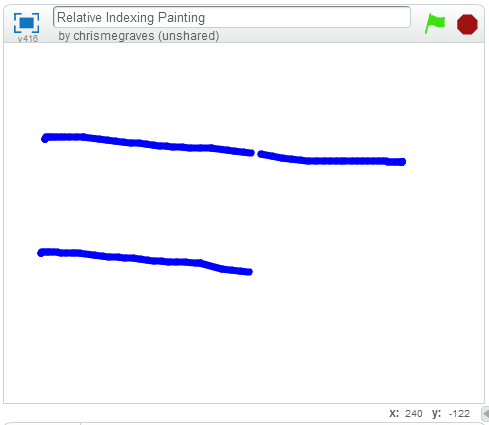
\includegraphics[width=0.5\textwidth]{images/IndexTransferGapBug.PNG}
\caption[Sample ``Wary" Script For Two-Finger Painting Using the Relative Indexing Design ]{On the left is a sample ``wary" script for the paintbrush using the Relative Indexing Design. On the right is the result of the bug that still exists in the ``wary" script.}
\label{WaryTwoFingerPaintingRID}
\end{figure}

\subsection{High Ceiling}

Since the Relative Indexing Design makes it impossible to practically implement a ``perfect" two-finger painting project, the same holds for the ten-finger painting project. Also, as the reader might imagine, the added logic needed to minimize (but not eliminate) the bugs in the two-finger project becomes much more convoluted when support for more fingers is added, because all touch index transfers must be accounted for. That being said, the level of complexity for the needed, additional logic is in line with the expected amount of difficulty for high ceiling projects. Although assembling the blocks would be tedious, the logic behind handling the transfers follows a pattern that can be repeated.

Similarly, the advanced two-player Pong game is quite difficult to implement using the Relative Indexing Design, but it can be done, and the amount of work and expertise needed is appropriate for a high ceiling project. Unlike the ten-finger painting project, however, the advanced two-player Pong game can be implemented exactly as specified with the Relative Indexing Design. The script for the advanced two-player Pong game paddle controls can be a little complicated (Figure \ref{AdvancedTwoPlayerPongRID}), but the logic is fairly straightforward. 

\begin{figure}
\centering
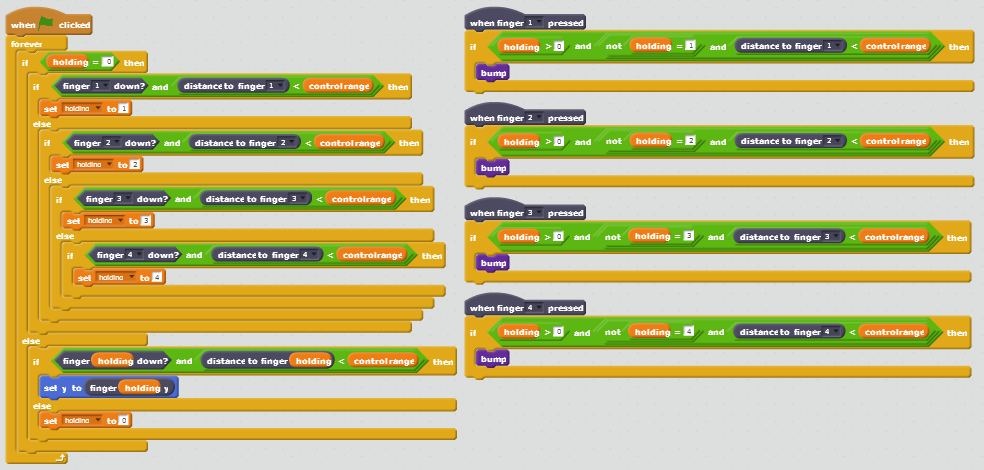
\includegraphics[width=1.0\textwidth]{images/AdvancedTwoPlayerPongRID.PNG}
\caption[Sample Relative Indexing Design Script For Advanced Two-Player Pong]{Here is a sample script for controlling the paddle in an advanced two-player Pong game using the Relative Indexing Design.}
\label{AdvancedTwoPlayerPongRID}
\end{figure}

The controls can be implemented using one ``forever loop" to control the movement and four ``when finger (\emph{index}) pressed" stacks to wait for bump-initiating taps. The ``forever loop" would first check if the paddle is currently following a finger. If the paddle is not following a finger, its script will query the touches with indices 1 through 4 (since we are assuming no more than four simultaneous touches) and decide to follow the first finger index it queries that is both down and within the paddle's control range. After deciding to follow a finger index, the paddle will follow that finger index until it is either lifted or moved out of range. 

The four ``when finger (\emph{index}) pressed" blocks will watch the finger indices 1 through 4. Their connected stacks will check for three criteria and, if they are met, will initiate a bump. The first criterion is that the paddle is currently following a touch. The second is that the touch being followed is not the touch that triggered the execution of the stack. Finally, the last criterion is that the touch that triggered the stack is within the paddle's control range.

As evidenced by the high ceiling case projects, the Relative Indexing Design does not make implementing complex projects particularly easy. However, the design does make their implementations possible (or at least almost possible, as is the case for the multi-finger painting projects). The intuitions for these implementations are almost always straightforward, but the actual assembly of the implementations can be tedious. Furthermore, there are subtle quirks with the Relative Indexing Design that are the basis for some tricky (albeit oftentimes surmountable) bugs.




